\documentclass[a4paper,14Q]{ltjsarticle}
\usepackage{graphicx}
\usepackage{wrapfig}
\usepackage[deluxe]{luatexja-preset}
\usepackage{tikz}
\usetikzlibrary{math,arrows.meta}
% \usepackage[notext]{stix2} 
\newcommand{\goshoku}[2]{#2}

\usepackage[explicit]{titlesec}
\titleformat{\section}[hang]{\Large\rmfamily\bfseries}{{\rmfamily\S\thesection.}}{4pt}{#1}[]% chktex 26 chktex 1

\newcommand{\maru}[1]{\raisebox{0.15ex}{\textcircled{\scalebox{0.9}{\raisebox{-0.2ex}{#1}}}}}
\newcommand{\syomonleftskip}{2\zw}
\newcommand{\toileftskip}{3\zw}
\newcommand{\shomon}[1]{\leftskip\syomonleftskip\hspace*{-1.5\zw}\llap{\bfseries(#1)}\hspace*{0.5\zw}}
\newcommand{\toi}[1]{\leftskip\toileftskip\hspace*{-1.5\zw}\llap{\bfseries#1.}\hspace*{0.5\zw}}
\newcommand{\MK}[1]{\setlength{\fboxrule}{0.8pt}\fboxsep2pt\framebox[2em]{\rmfamily\bfseries#1}}
\newcommand{\longMK}[1]{\setlength{\fboxrule}{0.8pt}\fboxsep2pt\framebox{\hspace*{0.3\zw}#1\hspace{0.3\zw}}}
\newcounter{num}
\newcommand{\options}[3][\quad]{
  \setcounter{num}{1}
  \bigskip\\#1
  \begin{tabular}{#2}
    #3
  \end{tabular}
}
\newcommand{\No}{\maru{\thenum}\stepcounter{num}\ }

\begin{document}
\noindent
{\Large\bfseries 力学2 確認テスト 2025/08/08(金)}\\[1.5\zh]
{\Large\sffamily\gtfamily 試験時間:\quad2限:10時25分\quad 〜\quad 11時25分\\[3\zh]
注意事項}\bigskip

\noindent\leftskip3\zw
\llap{(1)\quad}筆記用具、時計(時計機能だけのもの)、眼鏡、その他教員または監督員が認めたもの以外はすべてかばん等に入れること。
携帯電話、スマートフォン等は、電源を切り、かばん等に入れること(ただし、衣服に入れないこと)。\\
\llap{(2)\quad}机の中に何も入れないこと(自分のものではないものがあったら、担当教員または監督員に申し出ること)。\\
\llap{(3)\quad}試験開始の合図があるまで、答案用紙に記入してはならない。\\
\llap{(4)\quad}試験開始後20分は退室を認めない。\\
\llap{(5)\quad}試験時間中に担当教員または監督員の許可を得てトイレに行く際、スマートフォンを保持してはいけない。試験時間中、担当教員または監督員の許可無くスマートフォンを触ったら、不正行為とみなす。\\
\llap{(6)\quad}不正行為と疑われる行為は厳に慎むこと。
\par
なお、不正行為を行ったものには、学群学則及び筑波大学学群試験実施要項等に基づき、懲戒(停学等)の対象となる。
\vspace{2\zh}

\noindent\leftskip0\zw
{\large\bfseries マークシート記入上の注意:\\
  「氏名」「学籍番号」:}
\begin{center}
  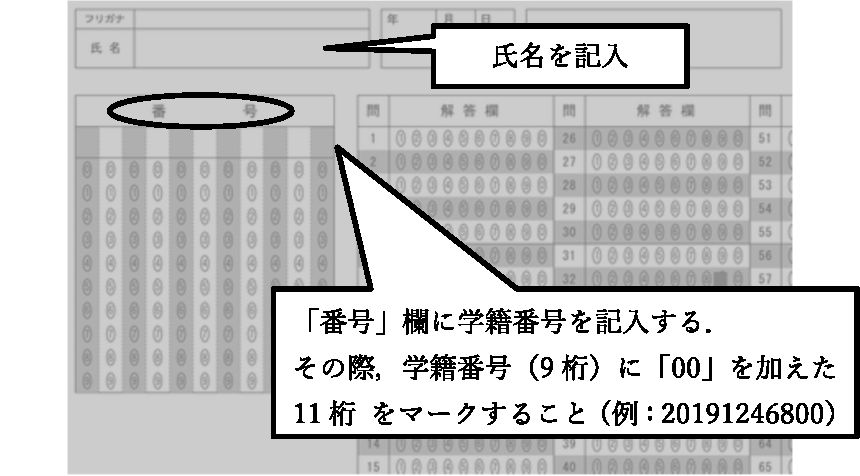
\includegraphics{hyo4fig.pdf}
\end{center}

\newpage
\section*{A.}\noindent
次の \longMK{空欄} に当てはまる言葉または数字を、各問題の選択肢から一つ選べ。
\bigskip

\shomon{1}物体をある力を受けながら始点から終点まで動かすときに要する仕事が、
始点と終点を結ぶ経路によらないとき、その力を \MK{1} という。
\options{llll}{\No 保存力 &\No 弾性力 &\No 摩擦力 &\No みかけの力}
\bigskip

\shomon{2}物体をある保存力を受けながら始点から終点まで動かすときに要する仕事は、始点と終点の \MK{2} の差になる。
\options{llll}{\No 重力エネルギー&\No 運動エネルギー&\No ポテンシャルエネルギー&\No 力積}
\bigskip

\shomon{3}ポテンシャルエネルギーと運動エネルギーの和を \MK{3} という。  
\options{ll}{\No 重力エネルギー&\No 運動エネルギー\\\No ポテンシャルエネルギー&\No 力学的エネルギー}
\bigskip

\shomon{4}保存力は、ポテンシャルエネルギーを \MK{4} することによって得られる。
\options{cccc}{\No 微分&\No 積分&\No 内積&\No 線績分}
\bigskip

\shomon{5}太陽のまわりをまわる惑星の運動は次の``ケプラーの法則''が成り立つ。\bigskip

\noindent\leftskip6\zw
\llap{第1法則}\ 惑星は太陽を \MK{5} の一つとする \MK{6} 軌道を描く。
\options[\hspace*{-2\zw}]{llll}{\No 中心&\No 重心&\No 焦点&\No 原点\\\No 直線&\No 平面&\No 楕円&\No 放物線}
\bigskip\\
\llap{第2法則}\ 惑星が太陽のまわりを単位時間にまわる \MK{7} と、惑星と太陽の距離の \MK{8} 乗をかけた値は一定である。
\options[\hspace*{-2\zw}]{lllll}{\No 角度&\No 距離&\No 速度&\No 角速度&\No 周期\\\No 2&\No 1/2&\No 3/2}
\newpage\noindent\leftskip6\zw
\llap{第3法則}\ 惑星が太陽のまわりをまわる \MK{9} は、楕円軌道の長半径の \MK{10} 乗に比例する。
\options[\hspace*{-2\zw}]{lllll}{\No 角度&\No 距離&\No 速度&\No 角速度&\No 周期\\\No 2&\No 1/2&\No 3/2}
\bigskip

\shomon{6}運動量は質量と \MK{11} の積で与えられるベクトル量であり、その時間微分は \MK{12} ベクトルである。
\options{lll}{\No 距離&\No 速度&\No 加速度\\\No 力&\No 力積&\No 力のモーメント}
\bigskip

\shomon{7}二物体の衝突の際、\MK{13} は常に保存される。\MK{14} 衝突の際には運動エネルギーも保存される。
\options{llll}{\No 運動量&\No 力学的エネルギー&\No 角運動量&\No 力積\\\No 弾性&\No 非弾性}
\bigskip

\shomon{8}質点系に働く重力の効果を考える際には、全重力が \MK{15} にはたらくとみなすことができる。
\options{llll}{\No 中心&\No 重心&\No 焦点&\No 原点}

\newpage\leftskip0\zw
\section*{B.}\noindent
二次元$xy$平面上で半径$R$の等速円運動質点を考えよう。質点の質量を$m$とする。時刻$t$での質点の位置が$x=R\cos\omega t,\,y=R\sin\omega t,\,z=0$であるとする。
\bigskip

\toi{16} この時、原点周りの角運動量として正しいものを以下から選べ。
\options{ll}{\No $\vec{l}=(0,0,mR^2\omega)$&\No $\vec{l}=-(0,0,mR^2\omega)$\\\No $\vec{l}=(mR^2\omega,mR^2\omega,mR^2\omega)$&\No $\vec{l}=-(mR^2\omega,mR^2\omega,mR^2\omega)$\\\No $\vec{l}=(mR^2\omega,mR^2\omega,0)$&\No $\vec{l}=-(mR^2\omega,mR^2\omega,0)$}

\section*{C.}\noindent
二次元$x,y$平面内の質点の運動を考えよう。質点の質量を$m$とする。質点の位置ベクトルを$\vec{r}=(x,y)$とする。
質点には中心力$\vec{F}=\vec{r}/r\cdot f(r)$が働いているとする。ここで、$r=|\vec{r}|$である。
\par\noindent
このとき、二次元極座標$r,\varphi\:(x=r\cos\varphi,\,y=r\sin\varphi)$を使って運動方程式がどのようになるか考えよう。
\bigskip

\shomon{1}動\goshoku{系}{径}方向の単位ベクトルを$\vec{e}_r$、$\varphi$方向の単位ベクトル$\vec{e}_\varphi$とする。
\par\noindent
$\vec{e}_x,\vec{e}_y$を\goshoku{x, y}{$x,y$}方向の単位ベクトルとするとき、$\vec{e}_r=\MK{17}$、$\vec{e}_\varphi=\MK{18}$の関係がある。
\par\noindent
\longMK{空欄} にあてはまる数式を以下から選べ。
\options{ll}{
\No $\phantom{-}\cos\varphi\,\vec{e}_x + \sin\varphi\,\vec{e}_y$ & \No $\phantom{-}\sin\varphi\,\vec{e}_x + \cos\varphi\,\vec{e}_y$\\
\No $\phantom{-}\cos\varphi\,\vec{e}_x - \sin\varphi\,\vec{e}_y$ & \No $\phantom{-}\sin\varphi\,\vec{e}_x - \cos\varphi\,\vec{e}_y$\\
\No $-\cos\varphi\,\vec{e}_x + \sin\varphi\,\vec{e}_y$ & \No $-\sin\varphi\,\vec{e}_x + \cos\varphi\,\vec{e}_y$}
\bigskip

\shomon{2}$\vec{e}_r$の時間微分は$\dot{\vec{e}}_r=\MK{19}$、$\vec{e}_\varphi$の時間微分は$\dot{\vec{e}}_\varphi=\MK{20}$である。
\par\noindent
\longMK{空欄}にあてはまる数式を以下から選べ。
\options{llll}{\No $\dot{\varphi}\vec{e}_\varphi$ &\No $-\dot{\varphi}\vec{e}_\varphi$ & \No $\dot{\varphi}\vec{e}_r$ & \No $-\dot{\varphi}\vec{e}_r$}
\bigskip

\shomon{3}\par
\toi{21}動径方向の運動方程式として正しいものを以下から選べ。
\options{ll}{
\No$m(\ddot{r}+r\dot{\varphi}^2)=f(r)$ &\No$m(\ddot{r}-r\dot{\varphi}^2)=f(r)$\\
\No$m(\ddot{r}+r\dot{\varphi}^2)=0$ &\No$m(\ddot{r}-r\dot{\varphi}^2)=0$}
\bigskip

\toi{22}角度方向の運動方程式として正しいものを以下から選べ。
\options{ll}{
\No$m(2\dot{r}\dot{\varphi}+r\ddot{\varphi})=f(r)$&\No$m(\dot{r}\dot{\varphi}+r\ddot{\varphi})=f(r)$\\
\No$m(2\dot{r}\dot{\varphi}+r\ddot{\varphi})=0$&\No$m(\dot{r}\dot{\varphi}+r\ddot{\varphi})=0$
}

\newpage\leftskip0\zw
\section*{D.}\noindent
太陽の周り\goshoku{}{を}回る惑星の公転周期$T$と、惑星の楕円運動の長半径$a$の間には、以下の関係がある\goshoku{}{。}
\par\noindent
(ケプラーの第三法則):$T^2=k\cdot a^3$。ここで$k$は定数である。
\bigskip

\toi{23}太陽の質量を$M$、惑星の質量を$m$、万有引力定数を$G$とする。この時定数$k$として正しいものを以下から選べ。
\options{llll}{
\No$2\pi^2/(Gm)$&\No$2\pi^2/(GM)$&\No$4\pi^2/(Gm)$&\No$4\pi^2/(GM)$\\
\No$2\pi^2m/(GM^2)$&\No$2\pi^2M/(Gm^2)$&\No$4\pi^2m/(GM^2)$&\No$4\pi^2M/(Gm^2)$}

\newpage\leftskip0\zw
\section*{E.}\noindent
\begin{wrapfigure}{r}[2\zw]{17\zw}
  \centering
  \vspace*{-15mm}
  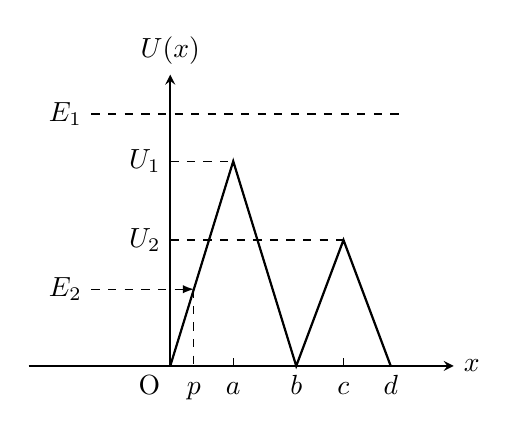
\begin{tikzpicture}[scale=0.1]
    \draw[semithick,->,>=stealth](-18,0)--(36,0)node[right]{$x$};
    \draw[semithick,->,>=stealth](0,0)node[below left]{O}--(0,37)node[above]{$U(x)$};
    \draw[thick](0,0)--(8,26)--(16,0)--(22,16)--(28,0);
    \draw[dashed](-10,32)node[left]{$E_1$}--(30,32);
    \draw[dashed](0,26)node[left]{$U_1$}--(8,26);
    \draw[dashed](0,16)node[left]{$U_2$}--(22,16);
    \draw[dashed,->,>=latex](-10,9.75)node[left]{$E_2$}--(3,9.75);
    \draw[dashed](3,9.75)--(3,0)node[below]{\phantom{$b$}$p$\phantom{$b$}};
    \draw(8,1)--(8,0)node[below]{\phantom{$b$}$a$\phantom{$b$}};
    \draw(16,0)node[below]{$b$};
    \draw(22,1)--(22,0)node[below]{\phantom{$b$}$c$\phantom{$b$}};
    \draw(28,0)node[below]{$d$};    
  \end{tikzpicture}
  \vspace{-15mm}
\end{wrapfigure}
$x$軸上で質量$m$の質点が、右図のように座標$a$と$c$にピークを持つ2つの山を有するポテンシャルエネルギーのもとで運動する場合を考える。
\par\noindent
$x=-\infty$の方向から質点が飛んでくるものとする。質点が持つ力学的エネルギーは、図に示される
$E_1$あるいは$E_2$の値のいずれかであるとする。以下の問いに答えよ。
\vspace{15mm}

\toi{24}$0<x<a$では質点にどのような力が働くか。
\options{lllllll}{\No$-\frac{U_1}{b}$&\No$\frac{U_1}{b}$&\No0&\No$-\frac{U_1}{a}$&\No$\frac{U_1}{a}$&\No$-\frac{U_1}{b-a}$&\No$\frac{U_1}{b-a}$}
\bigskip

\toi{25}$a<x<b$では質点にどのような力が働くか。
\options{lllllll}{\No$-\frac{U_1}{b}$&\No$\frac{U_1}{b}$&\No0&\No$-\frac{U_1}{a}$&\No$\frac{U_1}{a}$&\No$-\frac{U_1}{b-a}$&\No$\frac{U_1}{b-a}$}
\bigskip

\toi{26}質点が持つ力学的エネルギーが$E_1$の場合、$x<0$の範囲での速さはいくらか?
\options{llllll}{\No$\sqrt{\frac{2E_1}{m}}$&\No$\sqrt{\frac{E_1}{2m}}$&\No$\sqrt{\frac{E_1}{m}}$&\No0&\No$\frac{E_1}{m}$&\No$\frac{2E_1}{m}$}
\bigskip

\toi{27}質点が持つ力学的エネルギーが$E_1$の場合、$0<x<a$の範囲で質点の速さはいくらか?
\options{lll}{
  \No$\frac{1}{m}\left(E_1-\frac{U_1}{a}x\right)$ & \No$\frac{2}{m}\left(E_1+\frac{U_1}{a}x\right)$ & \No$\frac{2}{m}\left(E_1-\frac{U_1}{a}x\right)$\\
  \No$\sqrt{\frac{1}{m}\left(E_1-\frac{U_1}{a}x\right)}$ & \No$\sqrt{\frac{2}{m}\left(E_1+\frac{U_1}{a}x\right)}$ & \No$\sqrt{\frac{2}{m}\left(E_1-\frac{U_1}{a}x\right)}$
  }
\bigskip

\toi{28}質点の持つ力学的エネルギーが$E_1$の場合、$0<x$の範囲で質点の速さが最小となる座標はどこか?
\options{lllll}{\No$p$&\No$a$&\No$b$&\No$c$&\No$d$}
\bigskip

\toi{29}質点の持つ力学的エネルギーが$E_2$の場合、座標$p$での速さはいくらか?
\options{llllll}{\No$\sqrt{\frac{2E_2}{m}}$&\No$\sqrt{\frac{E_2}{2m}}$&\No$\sqrt{\frac{E_2}{m}}$&\No0&\No$\frac{E_2}{m}$&\No$\frac{2E_2}{m}$}

\newpage\leftskip0\zw\noindent
(下書き)





\end{document}